\chapter{Cơ sở lý thuyết}
\section{Giới thiệu}
Phát hiện từ khóa trong câu nói (KWS) là một nhiệm vụ quan trọng trong xử lý ngôn ngữ tự nhiên (NLP). KWS có thể được sử dụng trong nhiều ứng dụng khác nhau, chẳng hạn như tìm kiếm thông tin, tóm tắt văn bản, phân tích dữ liệu,...

Trong những năm gần đây, các phương pháp phát hiện từ khóa dựa trên deep learning đã được nghiên cứu và phát triển mạnh mẽ. Các phương pháp này có những ưu điểm vượt trội so với các phương pháp truyền thống như:

\begin{itemize}
    \item Có khả năng học hỏi từ dữ liệu lớn
    \item Có khả năng xử lý dữ liệu phức tạp
    \item Có thể phân biệt được các từ khóa quan trọng và các từ khóa không quan trọng
\end{itemize}

Các phương pháp phát hiện từ khóa dựa trên deep learning đã đạt được những thành tựu đáng kể trong những năm gần đây. Các phương pháp này đã được áp dụng thành công trong nhiều ứng dụng như tìm kiếm thông tin, tóm tắt văn bản, phân tích dữ liệu,...

Một số ứng dụng cụ thể của KWS bằng deep learning:
\begin{itemize}
        \item Tìm kiếm thông tin: KWS có thể được sử dụng để tìm kiếm thông tin từ các nguồn dữ liệu văn bản lớn, chẳng hạn như các trang web, các bài báo,... KWS có thể giúp người dùng tìm kiếm thông tin nhanh chóng và hiệu quả hơn.
        \item Tóm tắt văn bản: KWS có thể được sử dụng để tóm tắt nội dung của một văn bản dài. KWS có thể giúp người dùng hiểu nội dung của văn bản một cách nhanh chóng và dễ dàng hơn.
        \item Phân tích dữ liệu: KWS có thể được sử dụng để phân tích dữ liệu văn bản. KWS có thể giúp người dùng hiểu được các xu hướng và mối quan hệ trong dữ liệu văn bản.
\end{itemize}

\section{Các kiến trúc, mô hình và đặc trưng chưa được sử dụng}
\subsection{MFCC feature}

MFCC là viết tắt của Mel Frequency Cepstral Coefficient, là một kỹ thuật trích xuất đặc trưng phổ biến trong xử lý âm thanh và giọng nói. MFCC được sử dụng để biểu diễn các đặc tính phổ của âm thanh theo cách phù hợp với các bài toán học máy, như nhận dạng giọng nói và phân tích âm nhạc.

\begin{minipage}{\linewidth}
    \captionsetup{type=figure}
    \centering
    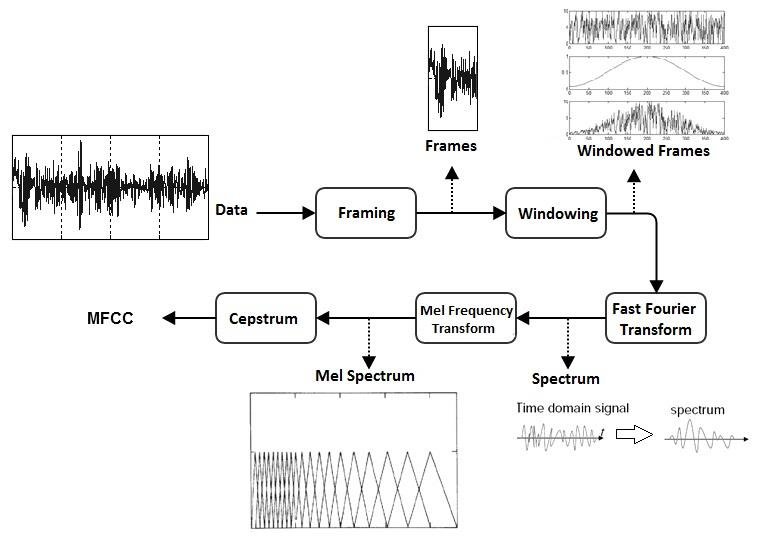
\includegraphics[width=0.9\textwidth]{images/mfcc.png}
    \caption{Sơ đồ rút trích đặc trưng MFCC}
\end{minipage}\par\vfill

MFCC được tính bằng cách biến đổi tín hiệu âm thanh từ miền thời gian sang miền tần số bằng một kỹ thuật như Biến đổi Fourier Rời rạc (DFT), sau đó áp dụng thang mel để xấp xỉ cách người nghe cảm nhận tần số âm thanh. Cuối cùng, hệ số cepstral được tính từ phổ mel.

MFCC có ích vì chúng nhấn mạnh các đặc trưng của tín hiệu âm thanh quan trọng cho cảm giác ngôn ngữ của con người, trong khi bỏ qua các thông tin ít liên quan hơn. Điều này làm cho chúng hiệu quả cho các bài toán như nhận dạng người nói, phát hiện cảm xúc và chuyển đổi giọng nói thành văn bản\cite{mfcc}.

\subsection{Kiến trúc seq2seq}

\begin{minipage}{\linewidth}
    \captionsetup{type=figure}
    \centering
    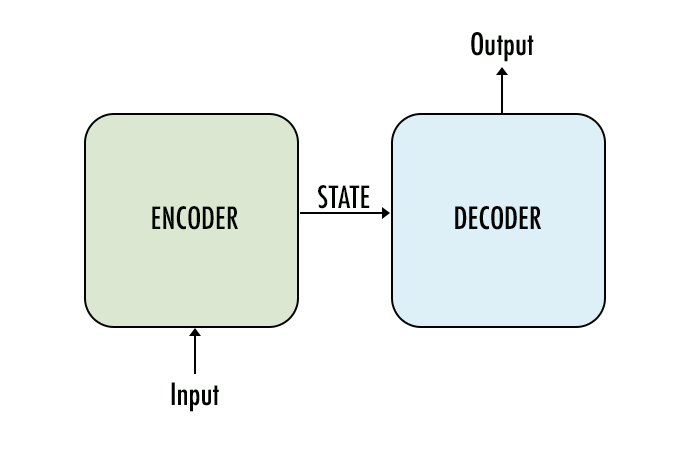
\includegraphics[width=0.9\textwidth]{images/seq2seq.png}
    \caption{Mô hình kiến trúc seq2seq}
\end{minipage}\par\vfill

Cách hoạt động:

\begin{enumerate}
    \item Bộ mã hóa: Bộ mã hóa sẽ quét chuỗi đầu vào từ trái sang phải, tại mỗi thời điểm, bộ mã hóa sẽ tạo ra một đại diện của từ hiện tại trong chuỗi đầu vào.
    \item Bộ giải mã: Bộ giải mã sẽ bắt đầu từ trạng thái đầu tiên của bộ mã hóa, tại mỗi thời điểm, bộ giải mã sẽ sử dụng đại diện trung gian được tạo ra bởi bộ mã hóa để tạo ra một từ trong chuỗi đầu ra.
\end{enumerate}

Kiến trúc seq2seq có những ưu điểm sau:
\begin{itemize}
    \item Có thể xử lý các chuỗi đầu vào và đầu ra có độ dài khác nhau.
    \item Có thể học hỏi các đặc trưng phức tạp của chuỗi đầu vào và đầu ra.
\end{itemize}

Kiến trúc seq2seq cũng có những nhược điểm sau:
\begin{itemize}
    \item Có thể yêu cầu nhiều tài nguyên tính toán, đặc biệt là đối với các chuỗi đầu vào và đầu ra có độ dài lớn.
    \item Có thể khó huấn luyện, đặc biệt là đối với các tập dữ liệu nhỏ.\cite{seq2seq} 
\end{itemize}

\subsection{Transformer}

Mô hình transformers là một kiến trúc mới trong lĩnh vực xử lý ngôn ngữ tự nhiên, được giới thiệu bởi bài báo “Attention is All You Need” năm 2017. Mô hình này sử dụng cơ chế attention để học biểu diễn của các từ trong ngữ cảnh của câu, và không cần dùng đến các mạng nơ-ron hồi tiếp (RNN) hay tích chập (CNN). 

\begin{minipage}{\linewidth}
    \captionsetup{type=figure}
    \centering
    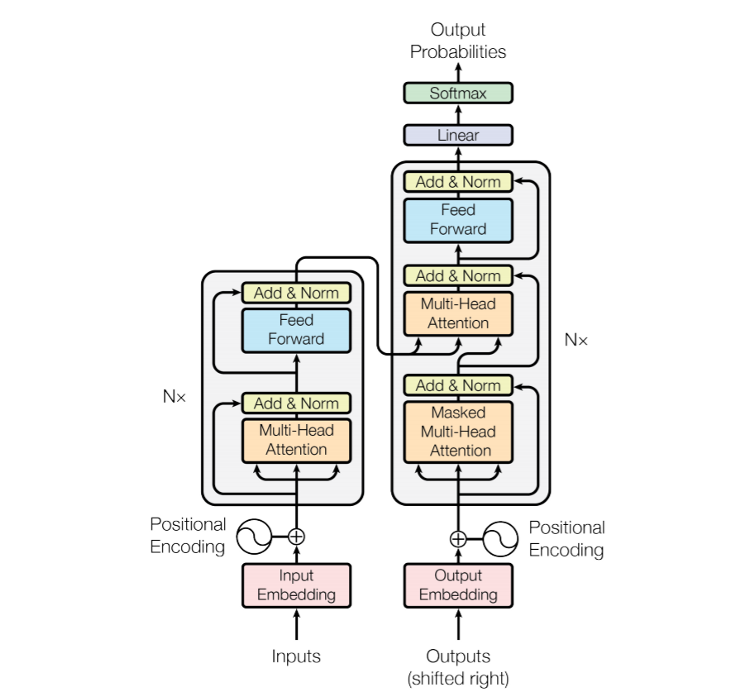
\includegraphics[width=0.7\textwidth]{images/transformer.png}
    \caption{Mô hình transformer}
\end{minipage}

Mô hình transformers gồm hai phần chính là encoder và decoder. Encoder nhận một câu ngôn ngữ nguồn và mã hóa nó thành một vector biểu diễn ngữ nghĩa. Decoder nhận vector biểu diễn này và dịch nó thành câu ngôn ngữ đích.

Cả encoder và decoder đều bao gồm nhiều tầng giống nhau, mỗi tầng gồm hai phần là self-attention và feedforward neural network. Self-attention cho phép các từ trong câu quan sát và tương tác với nhau để hiểu được mối quan hệ và ngữ cảnh của chúng. Feedforward neural network thực hiện các phép tính phi tuyến để học các đặc trưng của các từ. Ngoài ra, mô hình transformers còn sử dụng các kỹ thuật khác như position encoding, multi-head attention, residual connection và layer normalization để cải thiện hiệu suất và ổn định của mô hình.

Mô hình Transformer có những ưu điểm sau:

\begin{itemize}
    \item Có thể xử lý các chuỗi dữ liệu có độ dài khác nhau.
    \item Có thể học hỏi các đặc trưng phức tạp của chuỗi dữ liệu.
    \item Có thể đạt được hiệu quả cao hơn so với các kiến trúc mạng nơ-ron nhân tạo khác, chẳng hạn như RNN.
\end{itemize}

Mô hình transformers đã đạt được kết quả rất tốt trong nhiều bài toán xử lý ngôn ngữ tự nhiên.\cite{transformer}

\subsection{Pre-train model}

Pre-train model là một mô hình học máy đã được huấn luyện trước trên một tập dữ liệu lớn, thường là có tính đại diện cao, để có thể giải quyết nhiều bài toán.

\begin{minipage}{\linewidth}
    \captionsetup{type=figure}
    \centering
    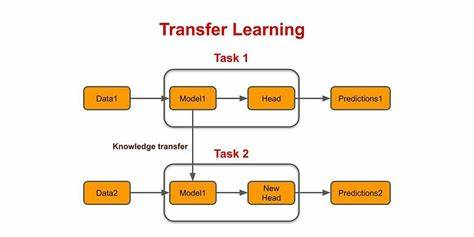
\includegraphics[width=0.7\textwidth]{images/pre-train-model.png}
    \caption{Kiến trúc mô hình fine tune}
\end{minipage}

Pre-train model có thể được sử dụng nguyên trạng hoặc được tinh chỉnh thêm để phù hợp với nhu cầu của ứng dụng cụ thể. Việc sử dụng Pre-train model trong KWS có nhiều lợi ích, như tiết kiệm thời gian, chi phí và công sức cho việc xây dựng mô hình từ đầu, tận dụng kiến thức đã học từ tập dữ liệu lớn, cải thiện hiệu suất và độ chính xác của mô hình, v.v…

Có nhiều kiểu Pre-train model trong KWS, nhưng một trong những kiểu phổ biến nhất là sử dụng các mô hình nhận dạng giọng nói tổng quát, như DeepSpeech, Wav2Vec hay QuartzNet, để làm backbone cho mô hình KWS. Các mô hình này đã được huấn luyện trước trên các tập dữ liệu lớn, như LibriSpeech hay Common Voice, để có thể nhận dạng bất kỳ từ nào trong tiếng Anh. Sau đó, các mô hình này được tinh chỉnh trên các tập dữ liệu nhỏ hơn, chỉ chứa các từ khóa cần phát hiện, để có thể phân biệt chúng với các từ khác\cite{pre-trained-models}.

\section{Các kiến trúc, mô hình và đặc trưng được sử dụng}
\subsection{Kiến trúc tổng thể}

Mô được sử dụng trong niên luận là một kiến trúc mạng nơ ron nhiều tầng nhiều lớp.

\begin{minipage} {\linewidth}
    \captionsetup{type=figure}
    \centering
    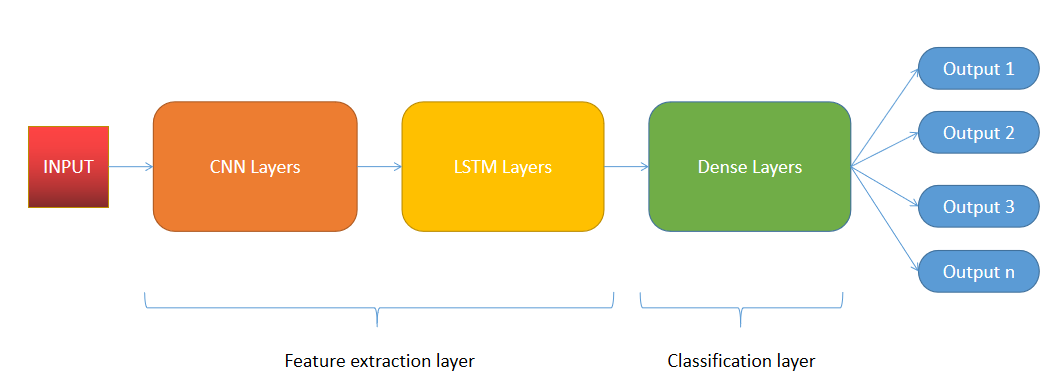
\includegraphics[width=1\textwidth]{images/kien_truc.png}
    \caption{Kiến trúc mô hình sử dụng}
\end{minipage}

Mô hình này có lớp chính là lớp trích xuất đặc trưng, lớp phân loại và các lớp phụ như lớp input, output. 

Lớp trích xuất đặc trưng: Bao gồm các lớp CNN và LSTM để học các đặc trưng không gian và thời gian từ dữ liệu đầu vào. Các lớp CNN sử dụng các bộ lọc để áp dụng các phép tích chập trên dữ liệu đầu vào và tạo ra các bản đồ đặc trưng. Các lớp LSTM sử dụng các ô nhớ để xử lý các chuỗi dữ liệu có độ dài biến đổi và học các mối quan hệ thời gian giữa các đặc trưng.

Lớp phân loại: Bao gồm các lớp dày đặc (dense) để giảm số chiều của đầu ra và học các biểu diễn trừu tượng của dữ liệu. Các lớp dày đặc kết nối đầy đủ với lớp trước đó và thực hiện một phép biến đổi tuyến tính trên đầu vào. Đầu ra của các lớp dày đặc có thể được truyền qua một hàm kích hoạt để giới thiệu tính phi tuyến.

Lớp đầu vào: Nhận dữ liệu đầu vào dưới dạng tensor có kích thước (chiều dài) và chuyển nó sang lớp trích xuất đặc trưng.

Lớp đầu ra: Tạo ra các giá trị đầu ra cho các mục tiêu khác nhau, ví dụ như phân loại. Lớp đầu ra là xác suất các từ xuất hiện trong câu.

\subsection{CNN}

Mạng nơ-ron tích chập (CNN), còn gọi là ConvNet, là một loại mạng nơ-ron nhân tạo (ANN), có kiến trúc cấp tiến sâu và có khả năng tổng quát hóa tuyệt vời so với các mạng khác có các lớp kết nối đầy đủ (FC), nó có thể học được các đặc trưng trừu tượng cao của các đối tượng đặc biệt là dữ liệu không gian và có thể nhận dạng chúng hiệu quả hơn.

Một mô hình CNN sâu bao gồm một tập hữu hạn các lớp xử lý có thể học được các đặc trưng khác nhau của dữ liệu đầu vào (ví dụ: ảnh) với nhiều cấp độ trừu tượng. Các lớp khởi tạo học và trích xuất các đặc trưng cấp cao (với trừu tượng thấp hơn), và các lớp sâu hơn học và trích xuất các đặc trưng cấp thấp (với trừu tượng cao hơn). Mô hình khái niệm cơ bản của CNN được thể hiện trong hình dưới, các loại lớp khác nhau được mô tả trong các phần tiếp theo\cite{cnn}.

\begin{minipage}{\linewidth}
    \captionsetup{type=figure}
    \centering
    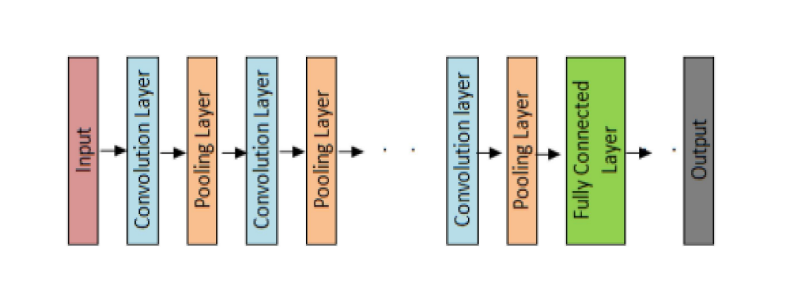
\includegraphics[width=1\textwidth]{images/concept_cnn.png}
    \caption{Khái niệm mô hình CNN}
    \label{fig:enter-label}
\end{minipage}

Một trong những lý do chính để xem xét CNN trong trường hợp này là tính năng chia sẻ trọng số của CNN, giúp giảm số lượng tham số có thể huấn luyện trong mạng, giúp mô hình tránh được hiện tượng quá khớp và cũng như cải thiện khả năng tổng quát hóa.

Trong CNN, lớp phân loại và các lớp trích xuất đặc trưng học cùng nhau, làm cho đầu ra của mô hình có tổ chức hơn và làm cho đầu ra phụ thuộc nhiều hơn vào các đặc trưng được trích xuất.

Việc triển khai một mạng lớn là khó khăn hơn bằng cách sử dụng các loại mạng nơ-ron khác thay vì sử dụng mạng nơ-ron tích chập. 

Ngày nay, CNN đã trở thành một cơ chế để đạt được kết quả hứa hẹn trong các ứng dụng dựa trên thị giác máy tính như phân loại ảnh, phát hiện đối tượng, phát hiện khuôn mặt, nhận dạng giọng nói, nhận dạng xe cộ, nhận dạng biểu cảm khuôn mặt, nhận dạng văn bản và đặc biệt trong bài toán KWS và nhiều bài toán khác.

Như đã đề cập trước đó, CNN bao gồm nhiều khối xây dựng (được gọi là lớp kiến trúc), trong phần này, sẽ mô tả chi tiết một số khối xây dựng này và vai trò của nó trong kiến trúc CNN.

\subsubsection{Convolutional Layer}

Lớp tích chập là thành phần quan trọng nhất của bất kỳ kiến trúc CNN nào. Nó chứa
một tập hợp các kernel (còn gọi là filter), được tích chập với đầu vào (Số liệu N chiều) để tạo output feature map.

\begin{enumerate}
    \item \textbf{Kernel: } \\
    Một kernel có thể được mô tả như một lưới các giá trị rời rạc hoặc số, trong đó mỗi giá trị được gọi là trọng số của kernel này. Khi bắt đầu quá trình huấn luyện của một mô hình CNN, tất cả các trọng số của một kernel được gán với các số ngẫu nhiên (cũng có các phương pháp khác để khởi tạo các trọng số). Sau đó, với mỗi epoch huấn luyện, các trọng số được điều chỉnh và kernel học cách trích xuất các đặc trưng có ý nghĩa. Trong hình dưới, chúng ta sẽ thấy một bộ lọc 2D. 
    
    \begin{minipage}{\linewidth}
        \captionsetup{type=figure}
        \centering
        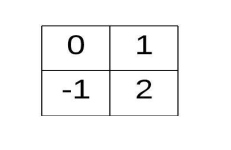
\includegraphics[width=0.25\textwidth]{images/kernel_example.png}
        \caption{Kernel 2D}
    \end{minipage}

    \item \textbf{Phép tích chập: } \\
    Trước khi đi sâu hơn, hãy cùng hiểu về định dạng đầu vào cho CNN. Không giống như các mạng nơ-ron cổ điển khác (nơi đầu vào là ở dạng vector), trong CNN đầu vào có thể là một ảnh đa kênh (ví dụ: đối với ảnh RGB như trong hình 1.8, nó có 3 kênh và đối với ảnh xám, nó có một kênh).\\
    
    \begin{minipage}{\linewidth}
            \captionsetup{type=figure}
            \centering
            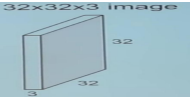
\includegraphics[width=0.5\textwidth]{images/image_rgb.png}
            \caption{Ảnh RGB 32x32}
    \end{minipage}

    Bây giờ, để hiểu về phép tích chập, nếu chúng ta lấy một ảnh xám kích thước 4 × 4, được hiển thị trong Hình 1.9 và một kernel 2 × 2 với các trọng số được khởi tạo ngẫu nhiên như trong Hình 1.10.
    \begin{figure}[h]
    \centering
    \begin{minipage}{0.45\textwidth}
        \centering
        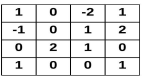
\includegraphics[width=0.9\textwidth]{images/image_gray.png} % first figure itself
        \caption{Ảnh xám 4x4}
    \end{minipage}\hfill
    \begin{minipage}{0.45\textwidth}
        \centering
        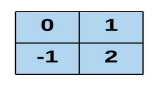
\includegraphics[width=0.9\textwidth]{images/kernel_2x2.png} % second figure itself
        \caption{Kernel 2x2}
    \end{minipage}
    \end{figure}

    Bây giờ, trong phép tích chập, chúng ta lấy kernel 2 × 2 và trượt nó trên toàn bộ ảnh 4 × 4 theo chiều ngang cũng như chiều dọc và trong quá trình đó chúng ta lấy tích vô hướng giữa kernel và ảnh đầu vào bằng cách nhân các giá trị tương ứng của chúng và cộng tất cả các giá trị để tạo ra một giá trị vô hướng trong bản đồ đặc trưng đầu ra. Quá trình này tiếp tục cho đến khi kernel không thể trượt thêm được nữa.

    Để hiểu rõ hơn, hãy xem một số phép tính ban đầu được thực hiện ở mỗi bước theo cách trực quan như trong Hình 1.11, nơi kernel 2 × 2 (màu xanh nhạt) được nhân với vùng cùng kích thước (màu vàng) trong ảnh đầu vào 4 × 4 và các giá trị kết quả được cộng lại để thu được một mục tương ứng (màu xanh đậm) trong bản đồ đặc trưng đầu ra ở mỗi bước tích chập.

    \begin{minipage}{\linewidth}
            \captionsetup{type=figure}
            \centering
            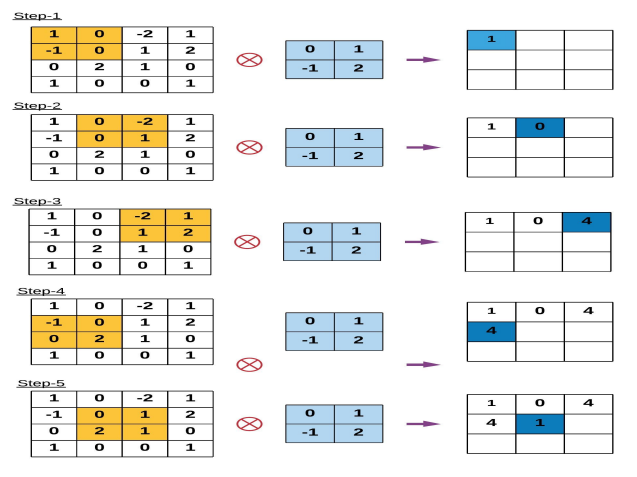
\includegraphics[width=0.9\textwidth]{images/conv.png}
            \caption{ Minh họa 5 bước đầu tiên của phép tích chập }
    \end{minipage}

    Sau khi thực hiện hoàn tất phép toán tích chập, bản đồ đặc trưng đầu ra cuối cùng được hiển thị trong Hình 1.12 như sau:
    
    \begin{minipage}{\linewidth}
            \captionsetup{type=figure}
            \centering
            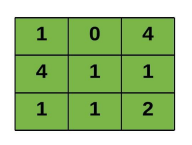
\includegraphics[width=0.5\textwidth]{images/feature_map.png}
            \caption{Bản đồ đặc trưng}
    \end{minipage}

    Lợi ích chính của các lớp tích chập bao gồm:
    \begin{itemize}
        \item Kết nối thưa: Trong một mạng nơ-ron hoàn toàn kết nối, mỗi nơ-ron của một lớp kết nối với mỗi nơ-ron của lớp tiếp theo nhưng trong CNN, chỉ có một số lượng nhỏ trọng số giữa hai lớp. Do đó, số lượng kết nối hoặc trọng số cần thiết là nhỏ, và lượng bộ nhớ để lưu trữ những trọng số này cũng nhỏ, vì vậy nó tiết kiệm bộ nhớ. Ngoài ra, phép toán dot(.) rẻ hơn về mặt tính toán so với phép nhân ma trận.
        \item Chia sẻ trọng số: Trong CNN, không có trọng số riêng biệt giữa hai nơ-ron của các lớp liền kề mà tất cả các trọng số hoạt động với từng pixel của ma trận đầu vào. Thay vì học trọng số mới cho mỗi nơ-ron, chúng ta có thể học một tập hợp trọng số cho tất cả các đầu vào và điều này giảm đáng kể thời gian đào tạo cũng như các chi phí khác.
    \end{itemize}
\end{enumerate}

\subsubsection{Pooling Layer}

Các lớp pooling được sử dụng để lấy mẫu con các bản đồ đặc trưng (được tạo sau các hoạt động tích chập), tức là nó lấy các bản đồ đặc trưng kích thước lớn hơn và thu nhỏ chúng thành các bản đồ đặc trưng kích thước thấp hơn. Trong khi thu nhỏ các bản đồ đặc trưng, nó luôn bảo tồn các đặc trưng (hoặc thông tin) chiếm ưu thế nhất trong mỗi bước pool. Hoạt động pooling được thực hiện bằng cách chỉ định kích thước vùng được pooled và sải bước của hoạt động, tương tự như hoạt động tích chập. Có các loại kỹ thuật pooling khác nhau được sử dụng trong các lớp pooling khác nhau như max pooling, min pooling, average pooling, gated pooling, tree pooling, v.v. Max Pooling là kỹ thuật pooling phổ biến nhất và được sử dụng nhiều nhất.

\begin{minipage}{\linewidth}
        \captionsetup{type=figure}
        \centering
        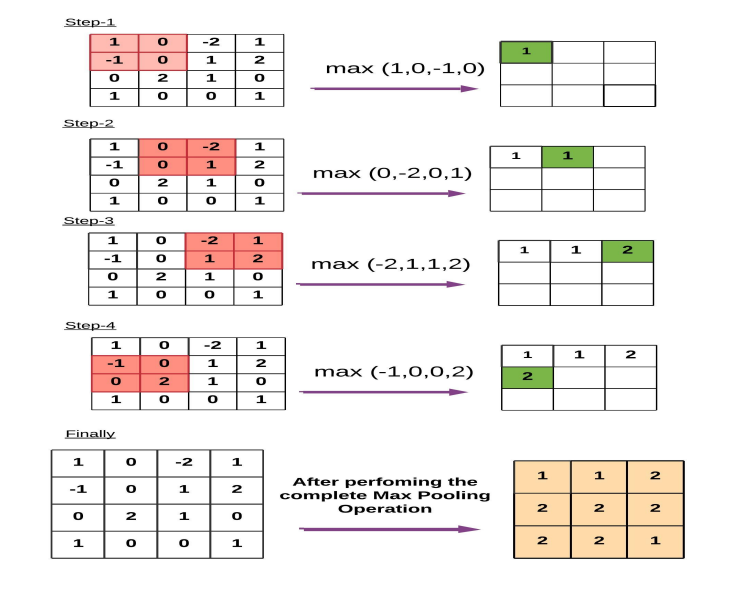
\includegraphics[width=0.9\textwidth]{images/pooling_layer.png}
        \caption{Minh họa một số bước ban đầu cũng như kết quả cuối cùng của phép MaxPooling, trong đó kích thước là 2 × 2}
\end{minipage}

\subsubsection{Hàm kích hoạt}

Nhiệm vụ chính của bất kỳ hàm kích hoạt nào trong bất kỳ mô hình dựa trên mạng nơ-ron nào là ánh xạ đầu vào thành đầu ra, nơi giá trị đầu vào được tính toán bằng cách tính tổng có trọng số của đầu vào nơ-ron và thêm bias vào đó (nếu có bias). Nói cách khác, hàm kích hoạt quyết định liệu một nơ-ron sẽ hoạt động hay không cho một đầu vào nhất định bằng cách tạo ra đầu ra tương ứng.

Trong kiến trúc CNN, sau mỗi lớp học được (các lớp có trọng số, tức là các lớp tích chập và FC) các lớp kích hoạt phi tuyến tính được sử dụng. Hành vi phi tuyến tính của những lớp này cho phép mô hình CNN học được nhiều thứ phức tạp hơn và quản lý để ánh xạ các đầu vào thành đầu ra theo cách phi tuyến tính. Đặc điểm quan trọng của một hàm kích hoạt là nó nên có thể phân biệt để cho phép lan truyền lỗi ngược để đào tạo mô hình. Các hàm kích hoạt được sử dụng phổ biến nhất trong các mạng nơ-ron sâu (bao gồm CNN) được mô tả dưới đây.

\begin{enumerate}
    \item \textbf{ReLU:}
    Hàm Rectifier Linear Unit (ReLU) là hàm kích hoạt được sử dụng phổ biến nhất trong Mạng Nơ-ron Tích chập. Nó được sử dụng để chuyển đổi tất cả các giá trị đầu vào thành số dương. Lợi ích của ReLU là nó chỉ yêu cầu rất ít tải tính toán so với những hàm khác. Biểu diễn toán học của ReLU là: \\
    $f(x)_{ReLU} = \max(0, x)$
    \begin{minipage}{\linewidth}
        \captionsetup{type=figure}
        \centering
        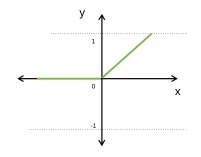
\includegraphics[width=0.5\textwidth]{images/relu.png}
        \caption{ReLU}
    \end{minipage}
    \item \textbf{Sigmoid:}
    Hàm kích hoạt sigmoid nhận số thực làm đầu vào và ràng buộc đầu ra trong phạm vi [0,1]. Đường cong của hàm sigmoid có hình dạng ‘S’. Biểu diễn toán học của sigmoid là:

    $f(x)_{sigmoid} = \frac{1}{1 + e^{-x}}$
    \begin{minipage}{\linewidth}
        \captionsetup{type=figure}
        \centering
        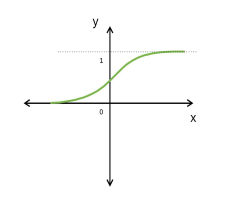
\includegraphics[width=0.5\textwidth]{images/sigmoid.png}
        \caption{Sigmoid}
    \end{minipage}

\end{enumerate}

\subsection{LSTM}

Mạng LSTM được cải tiến từ mạng thần kinh hồi quy (RNN–Recurrent Neural 
Network) nhằm khắc phục những nhược điểm về phụ thuộc xa (Long–term Dependency) của mạng RNN truyền thống. LSTM được giới thiệu bởi và càng ngày càng được cải tiến.

Về mặt lý thuyết, RNN có khả năng xử lý các phụ thuộc theo thời gian (temporal dependencies) bằng việc sử dụng bộ nhớ ngắn hạn và dựa trên việc xác định (luyện) các tham số một cách hiệu quả. Tuy nhiên, đáng tiếc trong thực tế RNN không thể giải quyết các phụ thuộc theo thời gian khi chuỗi số liệu có các phụ thuộc xa (long–term dependencies). Vấn đề này đã được nghiên cứu khá sâu bởi. Trong các công bố của mình, họ đã tìm được những lý do để giải thích tại sao RNN không thể học được một các hiệu quả.

LSTM có cấu trúc dạng chuỗi các nút mạng như RNN, nhưng cấu trúc bên trong thì lại phức tạp hơn, bao gồm 4 tầng tương tác với nhau (Hình 1.16). Điểm đặc biệt của mạng LSTM nằm ở trạng thái ô C (cell state), nơi lưu trữ các trọng số dài hạn của mô hình. Các thông số trạng thái ô C, trạng thái ẩn h (hidden state), đầu vào tại thời điểm t xt được đưa vào nút mạng. Sau khi được xử lý qua các hàm kích hoạt sigmoid, tanh và các phép toán véc–tơ, kết quả đầu ra là trạng thái ô C và trạng thái ẩn h tại thời điểm t sẽ được sử dụng cho nút mạng t+1 tiếp theo\cite{lstm}.

\begin{minipage}{\linewidth}
    \captionsetup{type=figure}
    \centering
    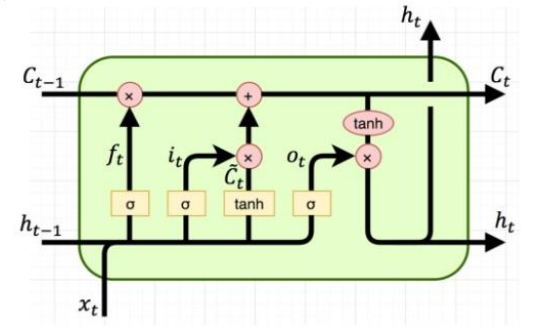
\includegraphics[width=0.5\textwidth]{images/lstm.png}
    \caption{Cấu trúc một nút mạng LSTM}
\end{minipage}




